\section{Introduction}
	\paragraph{}{
	As of 1996 in the United States and 2000 in the European Union, all vehicles must be fitted with an OBDII system. This system is detailed by a number of standards introduced by the Society of Automotive Engineers (SAE) and the California Air Resource Board (CARB). These standards define the hardware, software and communication requirements of the system.
	}
	\paragraph{}{
	All OBDII compliant vehicles must have an OBDII port (see figure \ref{fig:OBDport}). This a standardized 16 pin connector that is located within three feet of the driver seat, usually under the dashboard. This allows any generic diagnostic scan tool to connect to the vehicle and read data. While the connector is standardized, there are multiple communication protocols used by different manufacturers. These communication protocols provide the same data, but send it to the scan tool in a different format.
	}
	\paragraph{}{
	The OBDII port provides a connection to the ECU in the vehicle (see figure \ref{fig:ECU}). This is a computer that is connected to sensors and subsystems within the vehicle. These sensors are constantly monitoring the various aspects of the vehicle, such as engine speed and temperature. This data is sent to the ECU, allowing scan tools to read it. If these sensors detect that a data value is outside of the expected range, it may cause the malfunction indicator lamp (MIL) to be illuminated.
	}
	\begin{figure}[h]
		\begin{center}								
			\begin{minipage}{0.45\textwidth}
				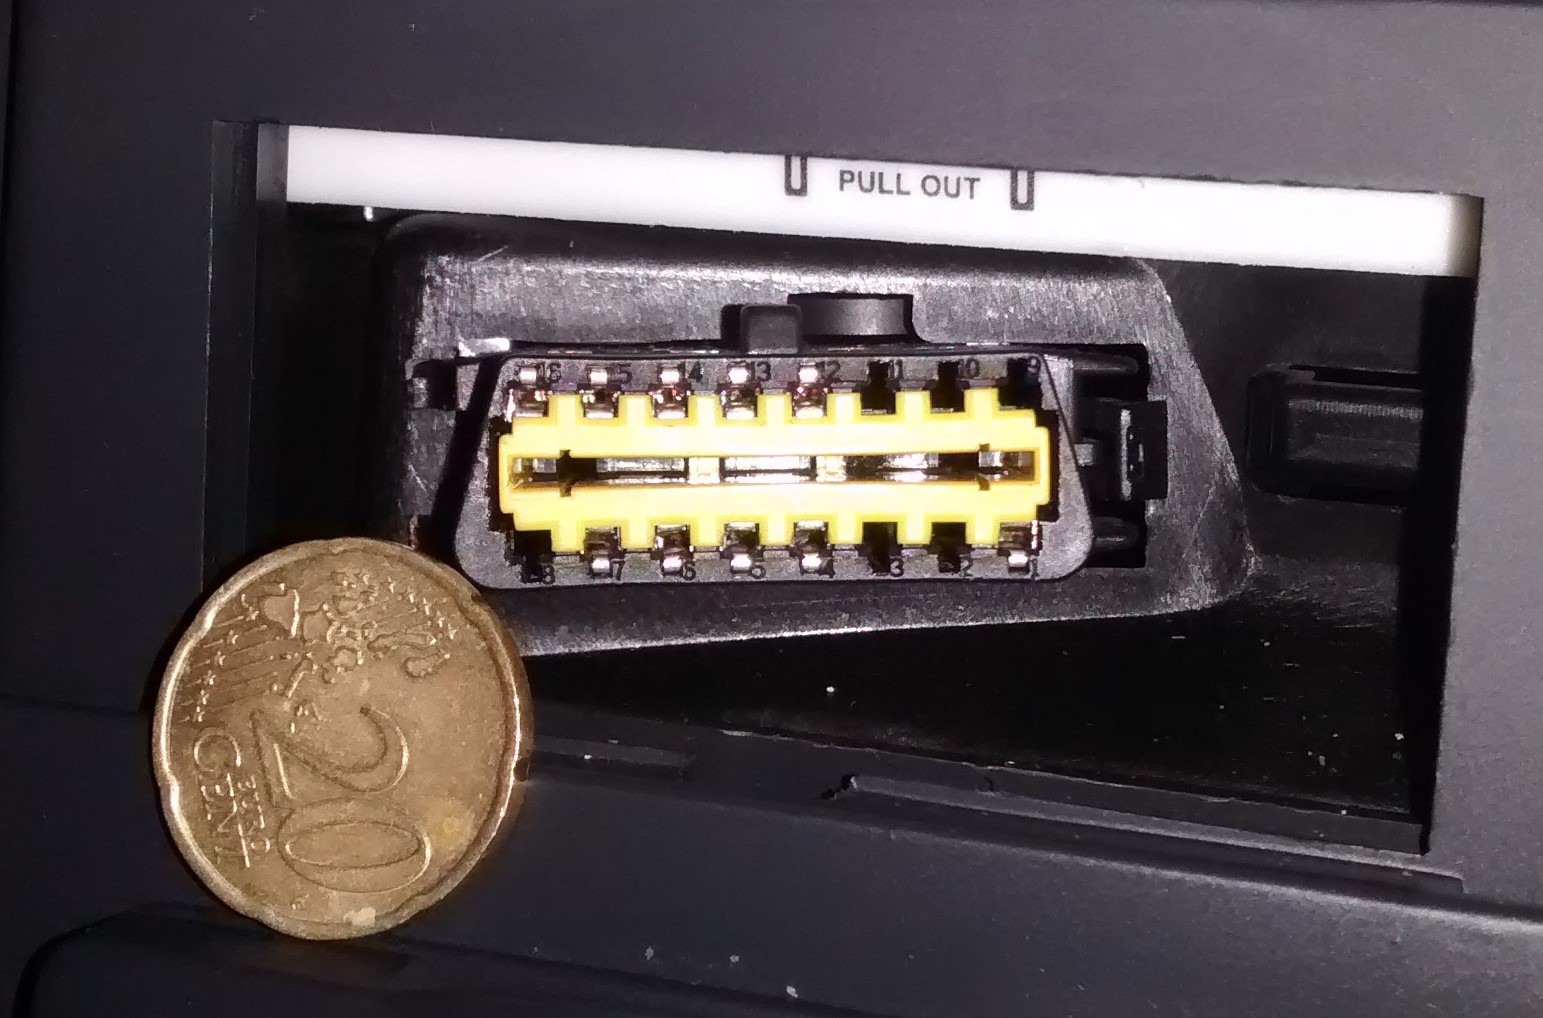
\includegraphics[width=\textwidth]{OBD.jpg}
				\caption{OBDII Port - 20 cent coin for scale}						
				\label{fig:OBDport}
			\end{minipage}
			\hfill			
			\begin{minipage}{0.45\textwidth}
				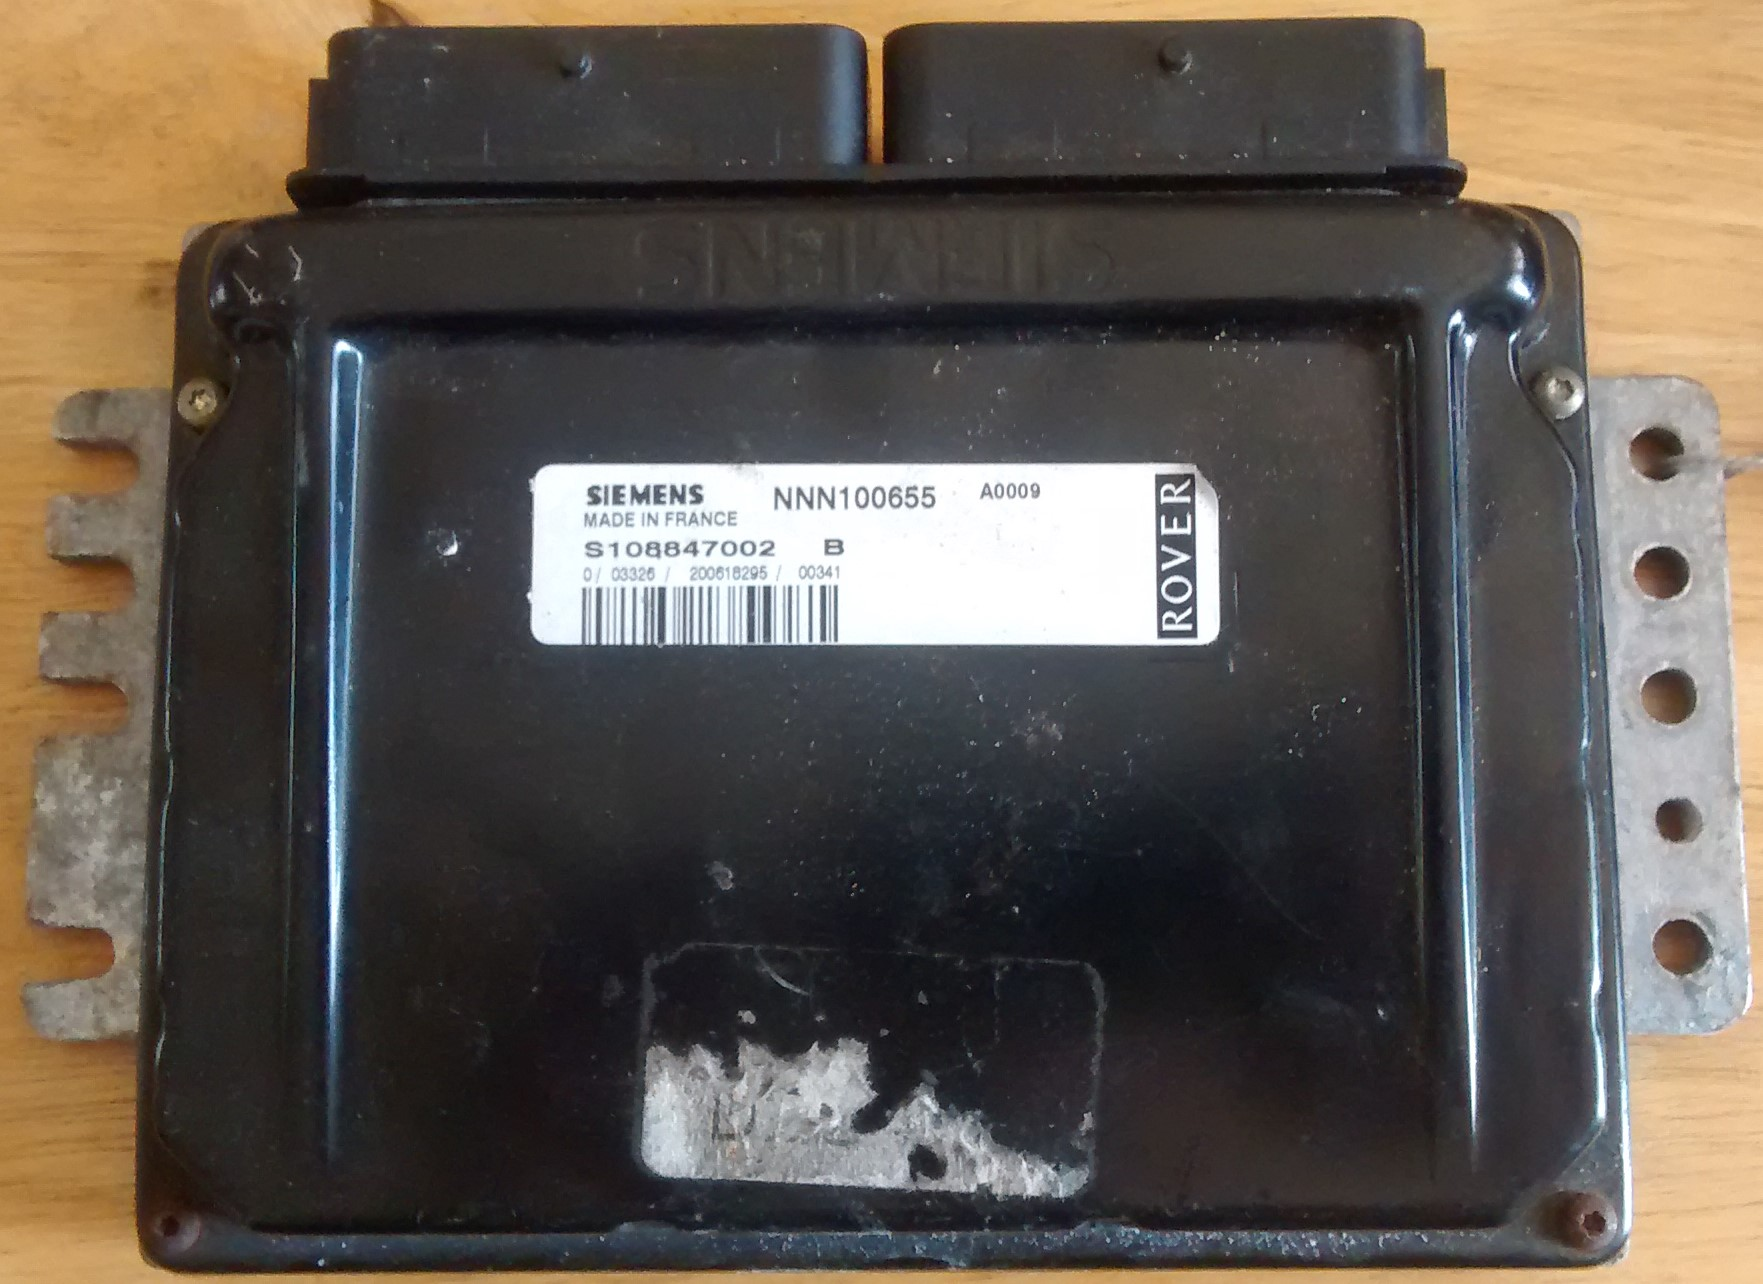
\includegraphics[width=\textwidth]{ECU.jpg}
				\caption{ECU - 20 cent coin for scale}
				\label{fig:ECU}
			\end{minipage}									
		\end{center}
	\end{figure}	
\newpage
\section{OBD Communication}
	\subsection{History}{
		\paragraph{}{
		Due to heavy smog pollution in California, CARB introduced regulations requiring all 1988 and newer vehicles sold in California to be fitted with a system for monitoring the emissions of the vehicle. Unfortunately, this system, later named OBDI, had its shortcomings. While new vehicles allowed for monitoring via diagnostic scan tools, the connection port and its position, as well as the communication protocols, were not standardized, meaning only proprietary scan tools could be used for diagnosis.
		}
		\paragraph{}{
		Prior to the introduction of OBDI, the SAE had proposed a standardised connection port and communication protocols. These changes were taken on board by CARB, and were introduced in OBDII, which was put in force in 1996 in the US. This new system, with it's standardised communication system allowed for generic scan tools to monitor for the vehicle, rather than just proprietary tools.  
		}	
		\paragraph{}{
		Eventually, these regulations reached Europe and European on board diagnostics (EOBD) was introduced. These regulations state that all petrols cars sold in Europe since 2001 and all diesel cars sold in Europe since 2003 must support EOBD. It should be noted that EOBD is the same as OBDII from a technical standpoint.
		}
		\paragraph{}{
		In 2008, regulations were introduced stating that all cars sold in the US must use the ISO 15765 Control Area Network (CAN) communication protocol. A communication protocol defines how data is transferred from the vehicle to the scan tool. This regulation will establish a standard method of communication for all future vehicles.
		}
	}	
	\subsection{Protocols}{
		\paragraph{}{
		The OBDII standards were lenient on how data is transmitted from the vehicle to the scan tool. This lead to vehicle manufacturers creating what they felt was the best way to handle communication. There are now five main communication protocols for OBDII systems.
		\begin{table}[h]
			\begin{center}				
				\begin{tabular}{| l | l |}
				\hline
				\textbf{Protocol} & \textbf{Manufacturer(s)}\\
				\hline
				J1850 Pulse Width Modulation (PWM) & Ford\\
				\hline
				J1850 Variable Pulse Width (VPW) & General Motors\\
				\hline
				ISO 9141-2 & Volkswagen, Audi\\
				\hline
				ISO 14230 Keyword Protocol 2000 (KWP2000) & Chrysler\\
				\hline
				ISO 15765 Control Area Network (CAN) & Toyota\\
				\hline			
				\end{tabular}
				\caption{OBD Protocols}
				\label{tab:Protocols}
			\end{center}
		\end{table}	
		}		
		\paragraph{}{
		Regardless of which protocol a vehicle uses, the process for requesting data is the same. The communication process is handled in hexadecimal format, and starts by selecting a mode. A mode represents a specific function to perform and there are ten in total from 01 to 0A. The functionality of each mode can be seen in table \ref{tab:Modes} and each will be discussed in sections \ref{ssec:DTC}, \ref{ssec:ClearCodes}, \ref{ssec:Data} and \ref{ssec:OtherModes}. Some modes require a parameter identifier (PID) to be passed, specifying the data item to retrieve. The ECU will send back a response and will have a different conversion method depending on the mode selected. The response will begin with the sum of the mode and $40 _{16}$, for example, if the user requested mode 03, the response would begin with 43.
		}
		\begin{table}[h]
			\begin{center}				
				\begin{tabular}{| l | l |}
				\hline
				\textbf{Mode} & \textbf{Description}\\
				\hline
				01 & Request current powertrain diagnostic data\\
				\hline
				02 & Request powertrain freeze frame data\\
				\hline
				03 & Request emission-related diagnostic trouble codes\\
				\hline
				04 & Clear/Reset emission-related diagnostic information\\
				\hline
				05 & Request oxygen sensor monitoring test results\\
				\hline
				06 & Request on-board sensor monitoring test results\\
				\hline
				07 & Request pending emission-related diagnostic trouble codes\\
				\hline
				08 & Request control of on-board system, test or component\\
				\hline
				09 & Request vehicle information\\
				\hline
				0A & Request permanent emission-related diagnostic trouble codes\\
				\hline
				\end{tabular}
				\caption{OBD Modes}
				\label{tab:Modes}
			\end{center}
		\end{table}		 
		
		\paragraph{}{
		Fortunately, most of the differences between these protocols are low level and do not impact how one can retrieve data from a vehicle using the defined commands. However, there are slight variations when using the CAN protocol.
		}
		\paragraph{}{
		 When requesting DTCs using the CAN protocol, response begins with the number of DTCs, followed by the hex values for each DTC. Using the other protocols, the response only contains the hex values for the DTCs. Mode 05 is unavailable using the CAN protocol so mode 06 must be used as an alternative method to access this data.
		}	
	}
	\subsection{Diagnostic Trouble Codes}{
		\paragraph{}{
		Diagnostic Trouble Codes (DTCs) correspond to faults with a vehicle and are responsible for the illumination of the MIL. Each code begins with an alphabetic letter, indicating the system at fault, followed by four digits specifying the fault. These systems are powertrain, chassis, body and network, represented by the characters P, C, B and U respectively. There are a number of standardized codes, but there are also manufacturer specific codes, which cannot be accessed with generic scan tools.
		}
		\paragraph{}{
		There are three types of DTC: stored, pending and permanent, accessed by mode 03, 07 and 0A respectively. Stored codes represent current issues with the vehicle. These codes can sometimes be fixed by calling the clear codes command on the scan tool. Pending codes represent potential future issues. If there is an irregular data value found by a sensor it may create a pending code. The ECU will continue to monitor this sensor, and if the data value has not returned to the expected value after a certain amount of time, the pending code is converted to a stored code. Otherwise, the pending code will be removed automatically. Permanent codes represent serious issues with the vehicle. These codes are not removed manually by scan tools or automatically by the ECU. In order to remove these codes, the underlying issue that caused the code to appear must be fixed.
		}			
	}
	\label{ssec:DTC}
	\subsection{Clear Codes}{
		\paragraph{}{
		The clear codes function allows one to clear all emissions-related diagnostic information from the ECU and can be accessed by mode 04. This removes stored and pending DTCs, on-board monitoring test results, oxygen sensor data, freeze frame data and data items pertaining to DTC and MIL information, such as distance travelled while MIL is activated.
		}
		\paragraph{}{
		In some cases, clear codes can turn off the MIL permanently. However, if the underlying issues are still present after the clear codes command has been sent, the MIL will illuminate again.
		}
	}
	\label{ssec:ClearCodes}
	
	\subsection{Data}{
		\paragraph{}{
		Emission related data can be accessed via mode 01. This data is retrieved from the sensors and subsystems of the vehicle. In this mode, the user must specify a PID in order to display a certain data item, for example, the PID 0C returns the engine speed.
		}
		\paragraph{}{
		The first step when requesting data is to find the PIDs that are supported for this vehicle, as some vehicles may only support a subset of PIDs. This can be achieved by using PIDs 00, 20, 40, 60 and 80, each of which represent the next 32 PIDs. This will return a hexadecimal value that, when converted to binary, denotes which PIDs are supported. Each bit in the binary string represents a PID. If the bit is 1, the PID is supported and if it is 0 the PID is unsupported.
						
		}
		\paragraph{}{
		As an example, we call 0120, to request the next 32 supported PIDs from 21 to 40. In this example, we receive the hexadecimal response \textit{1A300100}. When this response has been converted to binary, we get the following string:
		\begin{center}
			0001 1010 0011 0000 0000 0001 0000 0000\\
		\end{center}
		The most significant bit represents PID 21 and the least significant bit represents PID 40. If we look at the bits that are set to one, we determine that PIDs 24, 25, 27, 2B, 2C and 38 are supported.
		}
		\paragraph{}{
		Once the list of supported PIDs has been established, the user can request the data for these PIDs. This will return a single data value, so in order for the scan tool to display live data, it must repeat this call. The response must be converted from hexadecimal to the appropriate human readable value, either a string or number. Each PID has a different conversion method, although some PIDs may share them, for example engine coolant temperature and intake air temperature.
		}
	}
	\label{ssec:Data}
		
	\subsection{Other Modes}{
		\paragraph{}{
		Mode 02 allows access to freeze frame data. When a DTC is stored, the ECU takes a snapshot of the values for each available data item. This snapshot is known as freeze frame data. It is accessed and converted in the same way as PID data, although each data item only has one value. It can be used to pinpoint which component is at fault by checking for irregular data values.
		}		
		\paragraph{}{
		Mode 05 allows access to oxygen sensor monitoring test results. These sensors monitor the richness of the air/fuel mixture, which may affect the performance and fuel consumption of the vehicle. Mode 05 is no longer supported in the CAN protocol, but the data can be accessed via Mode 06 instead.
		}
		\paragraph{}{
		Mode 06 allows access to monitoring test results for specific components, such as catalyst monitoring. It can be used as an alternative to Mode 05 to access oxygen sensor monitoring. The user must pass a specific test identifier that is supported by the ECU. The method of finding the supported test identifiers is similar to the process of finding supported PIDs in Mode 02. 
		}
		\paragraph{}{
		Mode 09 allows access to vehicle information. The information available depends on the vehicle, but every vehicle has a vehicle identification number (VIN). This is a 17 character identifier unique to that vehicle, which can be used to search for the history of the vehicle. 
		}
	}
	\label{ssec:OtherModes}

\section{Technology}
	\subsection{ELM327}
		\paragraph{}{
		The ELM327 device (see figure \ref{fig:ELM327}) used for this project is a compact Bluetooth dongle that can connect to the OBDII port on modern vehicles. The device is relatively inexpensive, with the model used in this project costing {\textsterling}12.95. It supports all OBDII protocols and abstracts the data transfer process by including its own set of commands to handle communication.				
		}
		\paragraph{}{
		The commands that the device supports allow users to either manually or automatically select the protocol, depending on if they know which protocol their vehicle uses. These commands also handle initialization of the device, setting up communication, and formatting the data received from the vehicle. Once the device has been configured, the user can send requests to the vehicle. These requests are in the same format that they are found in the SAE J1979 document, and no further formatting is required.
		}
		\paragraph{}{
		The ELM327 device is easy to set up, without any technical knowledge. The communication set up is handled by the application that it is connected to, so the end user only has to connect the device to the vehicle and the computer that the application runs on. The device is also relatively inexpensive and easy to find on well known retail sites such as Amazon, so it is readily available for users who may not know of specialist retailers for diagnostic scan tools.
		}
		\begin{figure}[h]
				\begin{center}											
					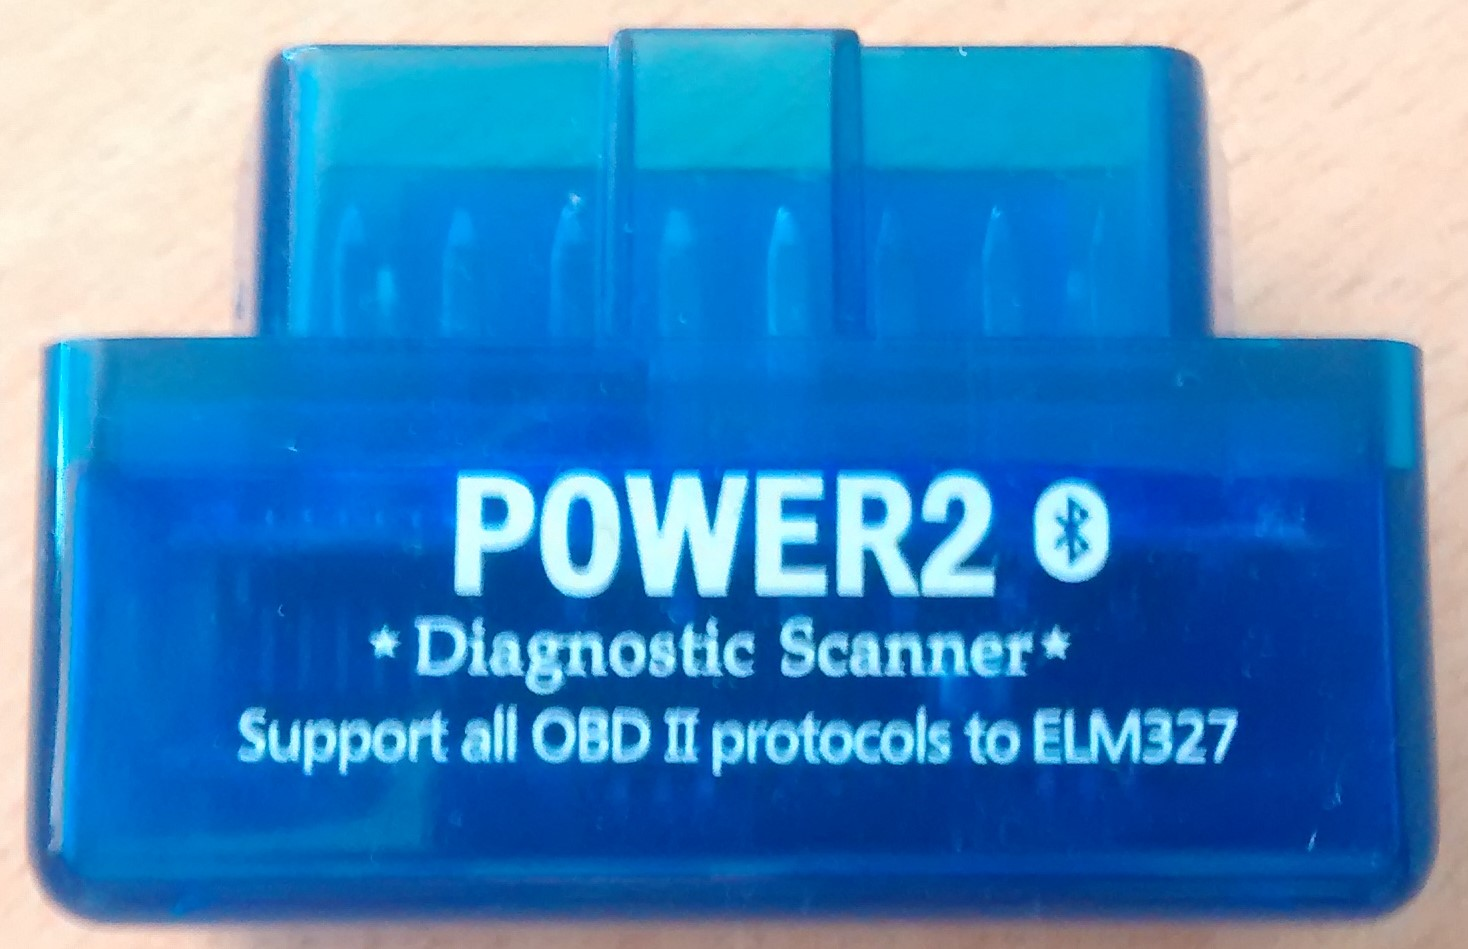
\includegraphics[width=0.4\textwidth]{ELM327.jpg}
					\caption{ELM327 Bluetooth Dongle}
					\label{fig:ELM327}
				\end{center}
		\end{figure}		
\newpage
	\subsection{Windows 10}
		\paragraph{}{
		This project will be deployed on Windows 10 using Microsoft's Universal Windows Platform (UWP). This will allow the application to be deployed on all Windows 10 devices, such as phones, tablets and laptops, using a single code base.
		}
		\paragraph{}{
		Windows is the de facto standard for home users. Most PCs and laptops are sold with Windows pre-installed. Windows 10, the latest iteration of the Windows operating system, is available as a free download to all owners of Windows 7 and Windows 8. Due to it's availability and pricing, it appears that Windows 10 may be a popular choice for home users, and as of October 2015 there are over 110 million devices running Windows 10.
		}
		\paragraph{}{
		With the release of Windows 10 came the Universal Windows Platform (UWP). This allowed developers to create applications that could be deployed on all Windows 10 devices, without having to create separate code bases. A similar concept was available in Windows 8.1, but it had it's limitations. Deployment was limited to Windows 8.1 phones and Windows 8 tablets/PCs, and there were separate code bases for the phone and desktop/tablet projects, making maintainability and extensibility of the system more complex.
		}
		\paragraph{}{
		The UWP also includes APIs for features such as Bluetooth, printing and WiFi. There is also extensive documentation available for these APIs, allowing the developer to implement systems that work across all devices with relative ease. Microsoft also provides design guidelines for UWP applications, allowing developers, who may not have an in depth knowledge of user interface and user experience design, to create applications with high usability that are aesthetically pleasing.
		}
		\paragraph{}{
		UWP applications can be published through the Windows Store that is accessible on all Windows 10 devices. This allows developers to reach a large user base without concerning themselves with the distribution of the application through multiple markets. Software updates can also be released through the Windows Store, ensuring new features and defect fixes can be deployed to the end user frequently and discreetly.
		}	
		
	\subsection{Xamarin}
		\paragraph{}{
		Xamarin is a framework that can be used for creating native applications for Android, iOS and Mac using the C{\#} programming language. This allows for native Windows applications to be ported to other operating systems, with minimal changes to the code base, creating a portable, extensible and maintainable system.
		}
		\paragraph{}{
		Xamarin allows developers to create applications with the same functionality and UI components of Android, iOS and Mac applications, using a C{\#} codebase. For example, Android UI elements such as buttons will appear and function in the same way as if they were created natively using Java. By creating a shared C{\#} library that contains the core functionality and then creating a platform specific presentation layer for each new operating system, it allows developers to target a large user base with a manageable codebase. 
		}
		\paragraph{}{
		Xamarin can be downloaded through the Visual Studio IDE, allowing Xamarin applications to be developed in the same IDE as the original C{\#} code. This benefits the developer, who does not have to track multiple projects over multiple IDEs. It also means any updates to the Xamarin framework can be downloaded seamlessly, without having to manually check if an update is available and downloading it from an external source. 
		}
		\paragraph{}{
		Xamarin has a developer community on their website, that provides assistance with the development of Xamarin applications. There are a number of guides ranging from the initial setup to performance best practises. Developers can also view Xamarin API documentation and sample applications on how to best use Xamarin and leverage the platform and device specific elements, such as the accelerometer and touch gestures. The website community also has a forum to post questions and find answers from other users, adding more support for the developer.
		}	
%\newpage
\section{Similar Applications}
	\paragraph{}{
	When looking at similar applications, it appeared preferable to look at applications developed using the same technology and deployed on the same platform that the project intended to use. This lead to finding two similar applications available on Windows 10 through the Windows Store. Investigation included finding which modes these applications included, their communication process, the hardware required and the amount of technical information used. These findings are presented in table \ref{tab:Features}.
	}
	
	\begin{table}[h]
		\begin{center}				
			\begin{tabular}{| l | c | c |}
			\hline
			\textbf{Function} & \textbf{Diagnose your car}  &\textbf{OBD dash}\\
			\hline
			Mode 01 & Yes & Yes\\
			\hline
			Mode 02 & &\\
			\hline
			Mode 03 & Yes & Yes\\
			\hline
			Mode 04 & &\\
			\hline
			Mode 05 & &\\
			\hline
			Mode 06 & &\\
			\hline
			Mode 07 & &\\
			\hline
			Mode 08 & &\\
			\hline
			Mode 09 & &\\
			\hline
			Mode 0A & &\\
			\hline
			Communication process & Bluetooth & Bluetooth\\
			\hline
			Device support & ELM327 & ELM327\\
			\hline			
			\end{tabular}
			\caption{Features of the similar applications}
			\label{tab:Features}
		\end{center}
	\end{table}
	
	\subsection{Diagnose your car}
		\paragraph{}{
		Diagnose your car is a Windows application available for Windows phones and PCs running Windows 8 and above. It is a paid application, with a free version available that removes some features and includes adverts. When discussing the application in this section, the focus will be on the PC version.
		}
		\paragraph{}{
		The application requires an ELM327 device and a PC capable of Bluetooth connection. The user can find information on the ELM327 in the application, such as where to buy it and how much it costs. The user must pair their ELM327 device with their PC before using the application. Once they have completed this step, they can connect to the device by entering the device name, and the application will automatically connect to it.
		}
		\paragraph{}{
		Diagnose your car allows access to DTCs and diagnostic data in the paid version. In the free version, diagnostic data is omitted and DTCs are displayed without their description. The diagnostic data that is provided is limited to a few generic PIDs, such as engine speed, vehicle speed and engine oil temperature. The data only displays the current value, so it does not track the data values over the period of communication. The application can also display DTCs, run the clear codes command and display the vehicle's VIN and the on/off status of the MIL.		
		}
		\paragraph{}{
		The application attempts to restrict its use of technical terms. For example, the DTCs option is named "Read Defects" and it's icon is that of the MIL, implying that this option correlates to turning off the MIL. However, when the user selects an option, the technical terms begin to appear, with defects now being called stored, pending and permanent DTCs, without an explanation of each type. 
		}		
	\subsection{OBD dash}
		\paragraph{}{
		OBD dash is a free Windows application available for PC. Like Diagnose your car, the application requires an ELM327 device and a PC capable of Bluetooth connection. Information on how to connect the ELM327 device to the vehicle and use it can be found within the application. The Bluetooth device must be paired with the PC before using OBD dash. The user can select their device from a list of suitable paired devices on opening the application.	
		%Modes included, Connection, UI etc
		}
		\paragraph{}{
		OBD dash allows access to DTCs, diagnostic data and vehicle information. PIDs are displayed in dials, similar to those found on the dashboard of a vehicle, and the user can add or remove the PIDs they want to monitor. However, only the current value is displayed, so multiple values cannot be compared over time. DTCs are displayed with their code as well as their description. However, only current and pending DTCs are available through the application. The application also allows the user to view the VIN and protocol that the vehicle supports.
		}
		\paragraph{}{
		Unlike Diagnose your Car, OBD dash uses technical terms frequently throughout the application. It refers to terms such as DTC and VIN without giving an explanation of what they are. While the application does include a help section that directs the user on how to use the application and configure the ELM327 device, it relies on the user having knowledge of protocols and OBD modes.
		%Technical terms
		}

\section{Architectural Patterns}
	\paragraph{}{
	When considering architectural patterns for the project, it made sense to utilise the model-view-viewmodel (MVVM) architectural pattern. The MVVM architectural pattern is based on Martin Fowler's presentation model design pattern and abstracts the user interface's state from it's behaviour. It was introduced by Microsoft in 2005 to be used with the Windows Presentation Foundation (WPF) platform and is used in UWP development.
			\begin{figure}[h]
				\begin{center}											
					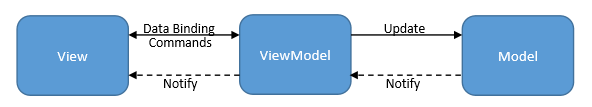
\includegraphics[width=\textwidth]{MVVM.png}
					\caption{Model-view-viewmodel diagram}											\label{fig:MVVM}
				\end{center}
			\end{figure}
	}
	\paragraph{}{
	The model represents the data to be displayed. An example of a model may be a stopwatch. The model can notify the viewmodel of any changes that have been made to the data, such as when the seconds on the stopwatch increase. Likewise, the viewmodel can also update the model with changes made by the view, such as pressing a reset button to set the timer to zero. It is important that the model does not contain logic relating to the user interface, such as formatting strings to appear more aesthetically pleasing.
	}
	\paragraph{}{
	The view represents the user interface and how the end user sees the data found in the model. It manages inputs and events, and notifies the viewmodel of these events. This is accomplished by data binding and commands, which allows properties and functions to be bound to certain UI elements, whilst also separating the logic from the view itself. In UWP, the view is created using Extensible Application Markup Language (XAML).
	}
	\paragraph{}{
	The viewmodel is the liaison between the view and the model. The view may want to update the model, or vice versa, and it must pass these requests to the viewmodel to be handled. For example, a  user may enter text into a field to set a property of the model. This field will be bound to a property on the viewmodel, that will then validate and format the data and pass it back to the model through exposed methods and properties.
	}	